\documentclass[11pt]{article}
\usepackage[cache=false]{minted}
\usepackage{amsmath} %used for maths and "aligned" in equation
\usepackage{hyperref}


\usepackage{tcolorbox}
\usepackage{etoolbox}
\BeforeBeginEnvironment{minted}%
     {\begin{tcolorbox}}%
\AfterEndEnvironment{minted}
   {\end{tcolorbox}}%


\usepackage{soul}
\definecolor{lightgray}{gray}{0.90}
\DeclareRobustCommand{\updated}[1]{{\sethlcolor{lightgray}\hl{#1}}}

\title{Algorithms}

\begin{document}
\maketitle

\tableofcontents

\section{Linked List}
We can use array to initialize the linked list as the following code.
While building up the linked list from the given array, we use the \textbf{two-pointer technique} to maintain the linking between two nodes.
\inputminted[breaklines=true,frame=leftline, linenos=true]{python}{src/linkedlist.py}

\section{Two Pointers Technique}
%TODO Two Pointers Technique
\subsection{Container With Most Water (LeetCode 11)}
Given $n$ non-negative integers $a_1$, $a_2$, ..., $a_n$ , where each represents a point at coordinate $(i, a_i)$. 
$n$ vertical lines are drawn such that the two endpoints of line $i$ is at $(i, a_i)$ and $(i, 0)$. 
Find two lines, which together with x-axis forms a container, such that the container contains the most water.

Note: You may not slant the container and $n$ is at least 2.

Example:
\begin{minted}[breaklines=true, xleftmargin=20pt]{bash}
Input: [1,8,6,2,5,4,8,3,7]
Output: 49
\end{minted}

\begin{figure}[h]
\centering
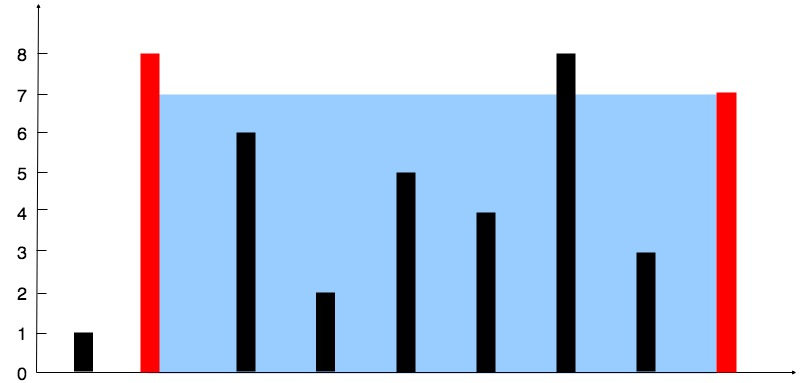
\includegraphics[width=8cm]{pic/question_11.jpg}
\caption{The above vertical lines are represented by array [1,8,6,2,5,4,8,3,7]. In this case, the max area of water (blue section) the container can contain is 49.}
\end{figure}


\section{Sliding Widow Technique}
\subsection{Count distinct elements in every window of size k}
Tag: Sliding Window Technique, Hashtable. 
See \footnote{https://www.geeksforgeeks.org/count-distinct-elements-in-every-window-of-size-k/}.

\begin{minted}[xleftmargin=20pt]{bash}
Input:  arr[] = {1, 2, 1, 3, 4, 2, 3}, k = 4
Output: [3, 4, 4, 3]
\end{minted}

We use the sliding window to update a hashtable, which maintains the distinct elements. And the time complexity is $O(n)$.

\inputminted{python}{src/distinct.py}

\subsection{Sliding Window Maximum (Maximum of all subarrays of size k)}

See \footnote{https://www.geeksforgeeks.org/sliding-window-maximum-maximum-of-all-subarrays-of-size-k/}.
\begin{minted}[xleftmargin=20pt]{bash}
Input :
arr[] = {1, 2, 3, 1, 4, 5, 2, 3, 6}
k = 3
Output :
3 3 4 5 5 5 6

Input :
arr[] = {8, 5, 10, 7, 9, 4, 15, 12, 90, 13}
k = 4
Output :
10 10 10 15 15 90 90
\end{minted}

We use the priority queue to .

\inputminted{python}{src/maxSlidingWindow.py}

\section{Heap}
Heap can be viewed as a complete tree, but stored as the array. 
Suppose the current node's index is $idx$, then the left child's index is $2*idx+1$, and the right child $2*idx+2$, while the parent $floor((idx-1)/2)$.

We take the binary max heap as an example. 
The basic external function is \textbf{insert} and \textbf{extractMax}, which is implemented by \textbf{siftup} and \textbf{siftdown}. 
The \textbf{siftup} function check the current node's value with its parent's value, then swap them if the current node's value is bigger than the parent's, and do the check-swap operation recursively to meet the guarantee 
	of the binary max heap.
	
The python source code is as following.
\inputminted[breaklines=true,frame=leftline, linenos=true]{python}{src/heap.py}

\subsection{Python's heapq}
We can use the library \textbf{heapq} in python. 
Since the default \textbf{heapq} is the min heap, so we need a trick to reimplement \textbf{MaxHeap} by overriding the comparison function. 
\inputminted[breaklines=true,frame=leftline, linenos=true]{python}{src/heap_heapq.py}

Or we can implement \textbf{MaxHeap} by multiplying -1 to each item in an array directly when using \textbf{heapq}.

\inputminted[breaklines=true,frame=leftline, linenos=true]{python}{src/heap_heapq2.py}

All the above three heap codes generate the following output. 
\begin{minted}[breaklines=true]{bash}
After inserting 1,2,3,4,5,6,7,8,9, the array of the heap is 9 8 6 7 3 2 5 1 4 .
Pop out from the heap, we'll get the maximum number 9, and the array of the heap becomes 8 7 6 4 3 2 5 1 .
\end{minted}

\subsection{The application of heap}
\subsubsection{Merge k Sorted Lists (LeetCode 23)}
Merge k sorted linked lists and return it as one sorted list. Analyze and describe its complexity\footnote{https://leetcode.com/problems/merge-k-sorted-lists/description/}.

\begin{minted}[xleftmargin=20pt]{bash}
Input:
[
  1->4->5,
  1->3->4,
  2->6
]
Output: 1->1->2->3->4->4->5->6
\end{minted}


\inputminted[breaklines=true,frame=leftline, linenos=true]{python}{src/mergeKSortedLists.py}

\subsubsection{Kth Largest Element in a Stream (LeetCode 703)}
Design a class to find the kth largest element in a stream. Note that it is the kth largest element in the sorted order, not the kth distinct element.

Your KthLargest class will have a constructor which accepts an integer k and an integer array nums, which contains initial elements from the stream. For each call to the method KthLargest.add, return the element representing the kth largest element in the stream.

Example:
\begin{minted}[xleftmargin=20pt]{bash}
int k = 3;
int[] arr = [4,5,8,2];
KthLargest kthLargest = new KthLargest(3, arr);
kthLargest.add(3);   // returns 4
kthLargest.add(5);   // returns 5
kthLargest.add(10);  // returns 5
kthLargest.add(9);   // returns 8
kthLargest.add(4);   // returns 8
\end{minted}

Note: 
\begin{enumerate}
	\item You may assume that nums' length $\geq k-1$  and $k \geq 1$.
\end{enumerate}

We use the min heap with the fixed size k to maintain the largest k elements in the stream. 
The minimum element in the min heap with size k will be the k-th largest element in a stream. 
The initialization of the heap is to heapify the given array.
Since the time complexity of the operation of "heapify" is $O(n)$\footnote{https://www.growingwiththeweb.com/data-structures/binary-heap/build-heap-proof/}, so the initialization is very efficient. 
And the add operation in the following code is to pop out the minimum element in the array which costs $O(\log k)$. 
In general, the time complexity is $O(n\log k)$, where $n$ is the size of the stream, and the space complexity is $O(\log k)$. 

\inputminted[breaklines=true,frame=leftline, linenos=true]{python}{src/kthLargestInStream.py}


\subsubsection{Top K Frequent Elements (LeetCode 347)}

Given a non-empty array of integers, return the k most frequent elements.

Example 1:
\begin{minted}[xleftmargin=20pt]{bash}
Input: nums = [1,1,1,2,2,3], k = 2
Output: [1,2]
\end{minted}

Example 2:
\begin{minted}[xleftmargin=20pt]{bash}
Input: nums = [1], k = 1
Output: [1]
\end{minted}

Note:
\begin{enumerate}
	\item You may assume k is always valid, $1 \leq k \leq $ number of unique elements.
	\item Your algorithm's time complexity must be better than $O(n \log n)$, where n is the array's size.
\end{enumerate}


There are two solutions for this problem: \textbf{min heap} and \textbf{max heap}. 
As the first solution, we use the \textbf{min heap} with the fixed size k to maintain the top k frequent elements, which is inspired by the problem \textbf{Kth Largest Element in an Array}.
Taking the counting frequent, heapifying the frequent-num array, and popping out the results into consideration, the time complexity is $O(n)+O(k+(n-k)\log k)+O(k \log k)$. 
So if $n \gg k$, the overall time complexity is $O(n \log k)$, but if $ n \approx k$, the overall time complexity is $O(n \log n)$.

\inputminted[breaklines=true,frame=leftline, linenos=true]{python}{src/topKFrequent.py}

As the second solution, we use the \textbf{max heap} to heapify the frequent-num tuples to a heap with the size $n$. 
Then we pop out the first $k$ elements in the max heap, which will be the result. Similar as the analysis on the min heap method, taking the counting frequent, heapifying the frequent-num array, and popping out the results into consideration, the time complexity is $O(n)+O(n)+O(k \log n)$. 
So if $n \gg k$, the overall time complexity is $O(n+k \log n)$ ($\approx O(n)$), but if $ n \approx k$, the overall time complexity is $O(n \log n)$.


\inputminted[breaklines=true,frame=leftline, linenos=true]{python}{src/topKFrequent_maxHeap.py}

\section{Tree}

\subsection{Univalued Binary Tree (LeetCode 965)}

A binary tree is univalued if every node in the tree has the same value.

Return true if and only if the given tree is univalued.

Example 1:
\begin{minted}[xleftmargin=20pt]{bash}
Input: [1,1,1,1,1,null,1]
Output: true
\end{minted}

Example 2:
\begin{minted}[xleftmargin=20pt]{bash}
Input: [2,2,2,5,2]
Output: false
\end{minted}

Note:
\begin{enumerate}
	\item The number of nodes in the given tree will be in the range [1, 100].
	\item Each node's value will be an integer in the range [0, 99].
\end{enumerate}

It's an easy problem. 
We use the recursion to get the result.
\inputminted[breaklines=true,frame=leftline, linenos=true]{python}{src/isUnivalTree.py}


\section{Sorting}
\subsection{Sort Characters By Frequency (LeetCode 451)}
Given a string, sort it in decreasing order based on the frequency of characters.

Example 1:
\begin{minted}[breaklines=true, xleftmargin=20pt]{bash}
Input:
"tree"

Output:
"eert"

Explanation:
'e' appears twice while 'r' and 't' both appear once.
So 'e' must appear before both 'r' and 't'. Therefore "eetr" is also a valid answer.
\end{minted}


Example 2:
\begin{minted}[breaklines=true, xleftmargin=20pt]{bash}
Input:
"cccaaa"

Output:
"cccaaa"

Explanation:
Both 'c' and 'a' appear three times, so "aaaccc" is also a valid answer.
Note that "cacaca" is incorrect, as the same characters must be together.
\end{minted}


Example 3:
\begin{minted}[breaklines=true, xleftmargin=20pt]{bash}
Input:
"Aabb"

Output:
"bbAa"

Explanation:
"bbaA" is also a valid answer, but "Aabb" is incorrect.
Note that 'A' and 'a' are treated as two different characters.
\end{minted}

This problem is not difficult. 
But we still should pay attention to the potential TLE problem may caused by the combination of string in python. 
We cannot use "s=s+c" which time complexity is $O(n^2)$ and space complexity is also $O(n^2)$ since it needs deep copy for every adding operation.

\inputminted[breaklines=true,frame=leftline, linenos=true]{python}{src/frequencySort.py}

\section{Dynamic Programming}

\subsection{Decode Ways (LeetCode 91)}
A message containing letters from A-Z is being encoded to numbers using the following mapping:
\begin{minted}[breaklines=true, xleftmargin=20pt]{bash}
'A' -> 1
'B' -> 2
...
'Z' -> 26	
\end{minted}
Given a non-empty string containing only digits, determine the total number of ways to decode it.

Example 1:
\begin{minted}[breaklines=true, xleftmargin=20pt]{bash}
Input: "12"
Output: 2
Explanation: It could be decoded as "AB" (1 2) or "L" (12).
\end{minted}

Example 2:
\begin{minted}[breaklines=true, xleftmargin=20pt]{bash}
Input: "226"
Output: 3
Explanation: It could be decoded as "BZ" (2 26), "VF" (22 6), or "BBF" (2 2 6).
\end{minted}

Firstly we use the Backtracking to search all the possible decoding ways, but failed to solve the problem with the \textbf{Time Limited Error}. 
The backtracking method is to decode the sequence like "1226..." in two ways: "1/226..." and "12/26...". 
Suppose the length of the input is $n$, the backtracking method's time complexity is $O(2^n)$ in worst case. 
A sequence of all one "$1 \cdots 1$" or all two "$2 \cdots 2$" are the worst cases. 

\inputminted[breaklines=true,frame=leftline, linenos=true]{python}{src/numDecodings.py}

Still consider the worst case "$1 \cdots 1$", which length is $n$. 
Suppose we have got the number of decoding ways for the subproblem "$1 \cdots 1 (n-1 \text{ ones})$" as $F(n-1)$ and the subproblem "$1 \cdots 1 (n-2 \text{ ones})$" as $F(n-2)$. 
Then the recursive formula is $F(n)=F(n-1)+F(n-2)$ for the worst case.

For the general cases "$c_1 c_2 c_3 \cdots c_{n-2} c_{n-1} c_{n}$", we should pay attention for the impossible decoding ways. 
Denote the number of decoding ways for the subproblem $c_1 \cdots c_{n-2}$ and the subproblem $c_1 \cdots c_{n-1}$.
We discuss the recursive formula in different conditions as follows.
\begin{enumerate}
	\item $c_{n-1}=0$ and $c_{n}=0$. The decoding way $c_1 c_2 c_3 \cdots c_{n-2}  0 | 0$ is not available, so $F(n)=0$.
	\item $c_{n-1}=0$ and $c_{n}\neq 0$. The decoding way $c_1 c_2 c_3 \cdots c_{n-2} | 0 c_{n}$ not available, but $c_1 c_2 c_3 \cdots c_{n-2}  0 | c_{n}$ is available, so $F(n)=F(n-1)$. 
	\item $c_{n-1}=1 \text{ or } 2$, and $c_{n}=0$. The decoding way is $c_1 c_2 c_3 \cdots c_{n-2}  | c_{n-1}  0$, so $F(n)=F(n-2)$.
	\item $c_{n-1}>=2$, and $c_{n}=0$. The decoding way is not available, so $F(n)=0$.
	\item $c_{n-1} \neq 0$ and $c_{n} \neq 0$, and $\text{int}(c_{n-1}c_{n})<=26$. Both two decoding ways are available, so $F(n)=F(n-1)+F(n-2)$.
	\item $c_{n-1} \neq 0$ and $c_{n} \neq 0$, and $\text{int}(c_{n-1}c_{n})>26$. Only the decoding way $c_1 c_2 c_3 \cdots c_{n-2} c_{n-1} | c_{n}$ can be applied, so $F(n)=F(n-1)$.
\end{enumerate}

\inputminted[breaklines=true,frame=leftline, linenos=true]{python}{src/numDecodings_dp.py}

\subsection{Decode Ways II (LeetCode 639)}
A message containing letters from A-Z is being encoded to numbers using the following mapping way:
\begin{minted}[breaklines=true, xleftmargin=20pt]{bash}
'A' -> 1
'B' -> 2
...
'Z' -> 26	
\end{minted}

Beyond that, now the encoded string can also contain the character '*', which can be treated as one of the numbers from 1 to 9.

Given the encoded message containing digits and the character '*', return the total number of ways to decode it.

Also, since the answer may be very large, you should return the output mod 109 + 7.

Example 1:
\begin{minted}[breaklines=true, xleftmargin=20pt]{bash}
Input: "*"
Output: 9
Explanation: The encoded message can be decoded to the string: "A", "B", "C", "D", "E", "F", "G", "H", "I".	
\end{minted}

Example 2:
\begin{minted}[breaklines=true, xleftmargin=20pt]{bash}
Input: "1*"
Output: 9 + 9 = 18	
\end{minted}

Note:
\begin{enumerate}
	\item The length of the input string will fit in range $[1, 10^5]$.
	\item The input string will only contain the character '*' and digits '0' - '9'.
\end{enumerate}

We start the analysis from the worst case "**...**(n times)", and from its simplest situation.
"*" represents 9 digits. 
And in "**", if the first star represents 1 or 2, then there are 32(=2*9+8+6) decoding ways; if the first star represents 3 to 9, then there are 63(=7*9) decoding ways. 
And in "***". 

\updated{TODO}
%TODO Decode ways II
\begin{enumerate} 
	\item $c_{n-1}=0$ and $c_{n}=0$. The decoding way $c_1 c_2 c_3 \cdots c_{n-2}  0 | 0$ is not available, so $F(n)=0$.
	\item $c_{n-1}=0$ and $c_{n}\neq 0$. The decoding way $c_1 c_2 c_3 \cdots c_{n-2} | 0 c_{n}$ not available, but $c_1 c_2 c_3 \cdots c_{n-2}  0 | c_{n}$ is available, so $F(n)=F(n-1)$. 
	\item $c_{n-1}=1 \text{ or } 2$, and $c_{n}=0$. The decoding way is $c_1 c_2 c_3 \cdots c_{n-2}  | c_{n-1}  0$, so $F(n)=F(n-2)$.
	\item $c_{n-1}>=2$, and $c_{n}=0$. The decoding way is not available, so $F(n)=0$.
	\item $c_{n-1} \neq 0$ and $c_{n} \neq 0$, and $\text{int}(c_{n-1}c_{n})<=26$. Both two decoding ways are available, so $F(n)=F(n-1)+F(n-2)$.
	\item $c_{n-1} \neq 0$ and $c_{n} \neq 0$, and $\text{int}(c_{n-1}c_{n})>26$. Only the decoding way $c_1 c_2 c_3 \cdots c_{n-2} c_{n-1} | c_{n}$ can be applied, so $F(n)=F(n-1)$.
\end{enumerate}


\section{Prefix Sum}
\subsection{What's Prefix Sum}
Given an array arr[] of size n, its prefix sum array prefixSum[] is the same size array such that prefixSum[i]=arr[0]+arr[1]+arr[2]+...+arr[i].
\subsection{Find if there is a subarray with 0 sum}

\begin{minted}[breaklines=true, xleftmargin=20pt]{bash}
Input: {4, 2, -3, 1, 6}
Output: true 
There is a subarray with zero sum from index 1 to 3.

Input: {4, 2, 0, 1, 6}
Output: true 
There is a subarray with zero sum from index 2 to 2.

Input: {-3, 2, 3, 1, 6}
Output: false
There is no subarray with zero sum.
\end{minted}

Solution: Use Prefix Sum method and HashMap used in Two Sum problem. 

\inputminted[breaklines=true,frame=leftline, linenos=true]{python}{src/subarraySum0.py}

The time complexity is $O(n)$.
The output of the running above code is as follows. 
Example:
\begin{minted}[breaklines=true, xleftmargin=20pt]{bash}
There are subarray in [4, 2, -3, 1, 6] such that its sum is 0, True or False? True
There are subarray in [4, 2, 0, 1, 6] such that its sum is 0, True or False? True
There are subarray in [-3, 2, 3, 1, 6] such that its sum is 0, True or False? False
\end{minted}

\subsection{Find the length of largest subarray with 0 sum}
Given an array of integers, find length of the largest subarray with sum equals to 0.
\begin{minted}[breaklines=true, xleftmargin=20pt]{bash}
Input: arr[] = {15, -2, 2, -8, 1, 7, 10, 23};
Output: 5
The largest subarray with 0 sum is -2, 2, -8, 1, 7

Input: arr[] = {1, 2, 3}
Output: 0
There is no subarray with 0 sum

Input: arr[] = {1, 0, 3}
Output: 1
\end{minted}

\inputminted[breaklines=true,frame=leftline, linenos=true]{python}{src/findLongestSubarraySum0.py}

The time complexity is $O(n)$.
The output of the running above code is as follows. 
Example:
\begin{minted}[breaklines=true, xleftmargin=20pt]{bash}
Length of the longest 0 sum subarray in [-3, 2, 3, 1, 6] is 0.
Length of the longest 0 sum subarray in [15, -2, 2, -8, 1, 7, 10, 13] is 5.
\end{minted}


\section{Maths}
\subsection{Prime numbers}
\subsubsection{Count Primes (LeetCode 204)}
Count the number of prime numbers \textbf{less than} a non-negative number, n.
Example:
\begin{minted}[breaklines=true, xleftmargin=20pt]{bash}
Input: 10
Output: 4
Explanation: There are 4 prime numbers less than 10, they are 2, 3, 5, 7.
\end{minted}

Tag: Primes.

We use the \textbf{Sieve of Eratosthenes} to label each number within the array of $[1, \cdots, n]$ is a prime or not.
\inputminted[breaklines=true,frame=leftline, linenos=true]{python}{src/countPrimes.py}

The line 18 to line 19 in the code can be optimized as the following code without the time consumption on the loop. 
\begin{minted}[breaklines=true, xleftmargin=20pt]{python}
primeFlags[p*p:n:p] = [False]*len(primeFlags[p*p:n:p])	
\end{minted}

By eliminating the inner loop, the time consumption is reduced from 860ms to 304ms. 

\subsubsection{Ugly Number (LeetCode 263)}
Write a program to check whether a given number is an ugly number.

Ugly numbers are positive numbers whose prime factors only include 2, 3, 5.

Example 1:
\begin{minted}[breaklines=true, xleftmargin=20pt]{bash}
Input: 6
Output: true
Explanation: 6 = 2 * 3
\end{minted}

Example 2:
\begin{minted}[breaklines=true, xleftmargin=20pt]{bash}
Input: 8
Output: true
Explanation: 8 = 2 * 2 * 2
\end{minted}

Example 3:
\begin{minted}[breaklines=true, xleftmargin=20pt]{bash}
Input: 14
Output: false 
Explanation: 14 is not ugly since it includes another prime factor 7.
\end{minted}

Note:
\begin{enumerate}
	\item 1 is typically treated as an ugly number.
	\item Input is within the 32-bit signed integer range: [$-2^{31}$, $2^{31}-1$].
\end{enumerate}

We use the while loop to do the check and the decomposition for a given number. Since the given number is within the range [$-2^{31}$, $2^{31}-1$], so we can do the check and the decomposition by recursion without worrying about the stack overflow (exceeding the maximum recursion depth). 
\inputminted[breaklines=true,frame=leftline, linenos=true]{python}{src/isUgly.py}

The recursion version is as following. 
\inputminted[breaklines=true,frame=leftline, linenos=true]{python}{src/isUgly_recursion.py}

\subsubsection{Ugly Number II (LeetCode 264)}
Write a program to find the n-th ugly number. 
Ugly numbers are positive numbers whose prime factors only include 2, 3, 5. 
Example:
\begin{minted}[breaklines=true, xleftmargin=20pt]{bash}
Input: n = 10
Output: 12
Explanation: 1, 2, 3, 4, 5, 6, 8, 9, 10, 12 is the sequence of the first 10 ugly numbers.
\end{minted}
Note:  
\begin{enumerate}
\item 1 is typically treated as an ugly number.
\item n does not exceed 1690.
\end{enumerate}

Tag: Maths, Primes, Tricky.

This problem's solution is very very tricky.
Although the tag on this problem includes dynamic programming. 
But I don't think it's a good example of the dynamic programming technique, because it can not get a clear \textbf{recursive formula}.
Instead, I would rather call it a tricky solution only using a tabulation. 

Suppose the resulted ugly number list is $F$. 
Since F includes the numbers whose factors only include 2, 3, and 5. 
So we build up three lists $l_2=2*F$, $l_3=3*F$, and $l_5=5*F$.
Therefore the ugly list $F$ has the property that $F=[1]+ merge(l_2,l_3,l_5)$.
Based on this property, what we should do is merging $l_2$, $l_3$, and $l_5$. 
The \textbf{tricky part} is that $F$ should be merged from $l_2$, $l_3$, and $l_5$, while these three lists are also need to be built from $F$.
We handle it by updating them simultaneously as the following code. 

\inputminted[breaklines=true,frame=leftline, linenos=true]{python}{src/uglyNumberII.py}

If we want to save the space of $l_2$, $l_3$, and $l_5$, then we'll do not claim space for them but use the space of $F$ only by maintaining the pointers in these three lists. The code is as following.
\inputminted[breaklines=true,frame=leftline, linenos=true]{python}{src/uglyNumberII_singleList.py}

%\begin{equation}
%	\begin{aligned}
%		F(n)=
%		\left\{ \begin{aligned}
%		1 &, n=1 & (a)\\
%		2 &, n=2 & (b)\\
%		3 &, n=3 & (c)\\
%		4 &, n=4 & (d)\\
%		5 &, n=5 & (e)\\
%		min\{2*F(n-3), 3*F(n-3), 5*F(n-3)\} &, n>5 & (f)
%		\end{aligned}\right.
%	\end{aligned}
%\end{equation}

\subsubsection{Super Ugly Number (LeetCode 313)}
Write a program to find the nth super ugly number.

Super ugly numbers are positive numbers whose all prime factors are in the given prime list primes of size k.

Example:
\begin{minted}[breaklines=true, xleftmargin=20pt]{bash}
Input: n = 12, primes = [2,7,13,19]
Output: 32 
Explanation: [1,2,4,7,8,13,14,16,19,26,28,32] is the sequence of the first 12 
             super ugly numbers given primes = [2,7,13,19] of size 4.
\end{minted}
Note:
\begin{enumerate}
	\item 1 is a super ugly number for any given primes.
	\item The given numbers in primes are in ascending order.
	\item $0 < k \leq 100$, $0 < n \leq 10^6$, $0 < \text{primes[i]} < 1000$.
	\item The nth super ugly number is guaranteed to fit in a 32-bit signed integer.
\end{enumerate}

Our solution is treat this problem as the extension of the problem \textbf{Ugly Number II}. 
This method's time complexity is $O(nk)$, where $k$ is the length of the array primes. 
But this method is not optimized, which should be speeded up to $O(n log k)$. 
Think about the problem \textbf{Merging k Sorted Lists}, which is optimized by using the data structure heap. 

\inputminted[breaklines=true,frame=leftline, linenos=true]{python}{src/nthSuperUglyNumber.py}

\subsection{Permutation}
\subsubsection{Next Permutation (LeetCode 31)}
Implement next permutation, which rearranges numbers into the lexicographically next greater permutation of numbers.

If such arrangement is not possible, it must rearrange it as the lowest possible order (ie, sorted in ascending order).

The replacement must be in-place and use only constant extra memory.

Here are some examples. Inputs are in the left-hand column and its corresponding outputs are in the right-hand column.
\begin{minted}[breaklines=true, xleftmargin=20pt]{bash}
1,2,3 -> 1,3,2
3,2,1 -> 1,2,3
1,1,5 -> 1,5,1	
\end{minted}


\end{document}
